\scanpage{18}
\uline{Ce foncteur est une équivalence de catégories.}

Pour prouver que $\mathcal L$ est un topos, le seul pb est de voir qu'il admet une petite famille génératrice. (Il est évident que $\mathcal L$ satisfait les conditions de Giraud a) b) c), et que $\omega$ \deleted{est} ex. à g. et commute aux $\underline{\lim}$). Dans le cas resp, $\mathcal L$ s'interprète comme la catégorie des \uline{sections cartésiennes} sur un topos fibré $F$ évident sur
\diagram{\begin{tikzcd}[ampersand replacement=\&]x'\arrow[r,bend left,"u"]\arrow[r,bend right,dash,"v"']\&x\end{tikzcd}},
\inserted{$F_{x'}=X',\quad F_x=X$,} associé aux changts de base $\alpha^*$, $\beta^*$, et on peut appliquer \inserted{SGA4} I 9.25. Dans le cas non resp, on \figure{\begin{tikzpicture}[x=1cm,y=1cm]
\node[anchor=north west] at (0,0) {\begin{minipage}{13cm}\deleted{\unsure{considère une catégorie}\ \inserted{topos fibré $F$ sur}
\diagram{\begin{tikzcd}[ampersand replacement=\&]x'\arrow[d,"f"']\arrow[dr,"u"]\&\\x'_1\arrow[r,"v"']\&x\end{tikzcd}}
\unsure{associé aux changts de base $u$}}\end{minipage}};
\draw (1.3,.02)--(12.9,.1)--(9.4,.28)--(9.3,.49)--(7.7,.43);
\draw (1.3,.02)--(1.25,-1.6) (1.22,-1.72)--(1.15,-2.5)--(.05,-2.6)--(.05,-2.95)--(8.45,-2.75) to[out=0,in=-60] (8.7,-2.25) to[out=120,in=-90] (7.5,-.22);
\end{tikzpicture}}
\unsure{remarque} que les arguments de SGA4 I 9.21 et suite donnent le résultat \unsure{.....|voulu}.
\margin{\uline{à vérifier}}

\figure{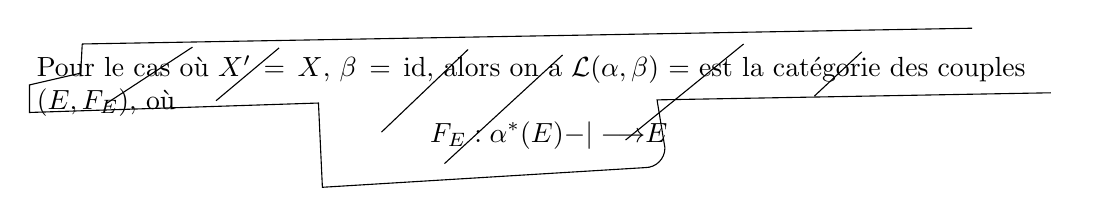
\begin{tikzpicture}[x=1cm,y=1cm]
\node[anchor=north west,text width=13cm,align=left] at (0,0) {\deleted{\unsure{Pour le cas où} $X'=X$, $\beta=\mathrm{id}$, alors \unsure{on a} $\mathcal L(\alpha,\beta)$ \deleted{\unsure{=}} est la catégorie des couples $(E,F_E)$, où
\[
F_E:\alpha^*(E)\unsure{-|\longrightarrow}E
\]}};
\draw (.7,.02)--(12,.22);
\draw (.7,.02)--(.68,-.35)--(.03,-.5)--(.03,-.85)--(3.7,-.73)--(3.75,-1.8)--(7.85,-1.55) to[out=0,in=-90] (8.1,-1.3)--(8.0,-.69)--(13,-.6);
\draw (1.0,-.74)--(2.1,-.02) (2.4,-.7)--(3.2,-.03) (4.5,-1.1)--(5.6,-.05) (5.3,-1.5)--(6.8,-.12) (7.6,-1.2)--(9.1,.02) (10,-.64)--(10.6,-.08);
\end{tikzpicture}}

Le \deleted{catégorie} \inserted{topos} $\mathcal L(\alpha,\beta)$ dépend ``fonctoriellement'' de
\diagram{\begin{tikzcd}[ampersand replacement=\&]\alpha,\beta:\quad X'\arrow[r,shift left]\arrow[r,shift right,dash]\&X\end{tikzcd}}
de façon précise, si on a un diagramme
\diagram{\begin{tikzcd}[ampersand replacement=\&]
u:\quad X'\arrow[r,shift left,"\alpha"]\arrow[r,shift right,dash,"\beta"']\arrow[d,"u_1"']\arrow[dr,phantom,"\unsure{\nearrow\ \nearrow|\xi\ \psi}" description]\&X\arrow[d,"u_0"]\\
Y'\arrow[r,shift left,"\lambda"]\arrow[r,shift right,dash,"\mu"']\&Y
\end{tikzcd}}
\margin{\unsure{a|u}}
\mspage{17}
